\documentclass{article}
\usepackage{amsmath}
\usepackage{amssymb}
\usepackage{amsfonts}
\usepackage{dsfont}
\usepackage{graphicx} % Required for inserting images
\usepackage{listings}
	\lstset{language=R,
    basicstyle=\small\ttfamily,
    stringstyle=\color{green},
    otherkeywords={0,1,2,3,4,5,6,7,8,9},
    morekeywords={TRUE,FALSE},
    deletekeywords={data,frame,length,as,character},
    keywordstyle=\color{blue},
    commentstyle=\color{green},
}
\usepackage{xcolor}
\usepackage{array}
\usepackage[vmargin=2cm,hmargin=2cm]{geometry}


\title{TP2-ADM}
\author{Guillaume Bernard-Reymond et Lorenzo Gaggini}
\date{Décembre 2023}

\begin{document}
\newcommand{\norme}[1]{\left\| #1\right\|}
\newcommand{\tr}{\text{tr}}
\maketitle
\setlength{\parindent}{0pt}

Dans ce TP, nous avons à notre disposition un jeu données concernant 100 villes françaises dont on connaît 54 indicateurs répartis en quatre grands thèmes : Economie, Risques, Nature et Culture.\\

Nous avons décidé d'utiliser la bibliothèque Factoshiny pour son confort d'utilisation. 

\section{ACP normé sur l'ensemble des variables}

\subsection{Etude de la variance cumulée}

Dans un premier temps, nous nous intéressons à la variance cumulée et notamment les grands décrochements. Nous allons devoir faire un choix qui ne sera malheureusement pas sans perte d'informations.

Voici le graphique des valeurs des valeurs propres : 

\centerline{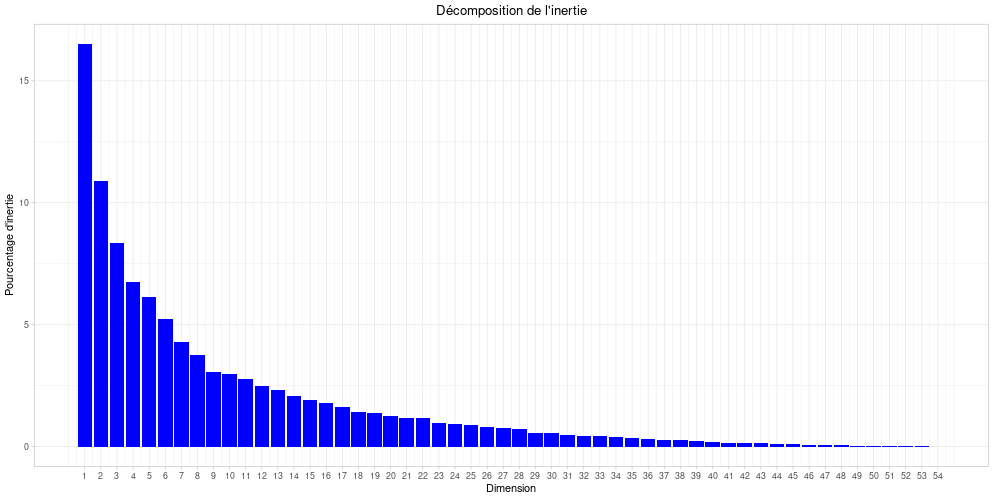
\includegraphics[width=\linewidth]{images/ACP_vp}} 

Voici le tableau des variances cumulées :

\begin{center}
 \begin{tabular}{|l|*{8}{>{\centering\arraybackslash}p{1cm}|}}
 \hline 
 \rule[-1ex]{0pt}{2.5ex} Valeurs propres & Dim.1  & Dim.2 &  Dim.3 &  Dim.4 &  Dim.5 &  Dim.6 &  Dim.7 & Dim.8\\ 
 \hline 
 \rule[-1ex]{0pt}{2.5ex}  Variance & 8.914 &  5.889  & 4.511 &  3.646  & 3.306 &  2.820  & 2.326 & 2.041\\
 \hline 
 \rule[-1ex]{0pt}{2.5ex} 
$\%$ of var. &  16.508 & 10.906 &  8.353 &  6.752  & 6.121 &  5.222 &  4.307 & 3.780 \\
 \hline 
 \rule[-1ex]{0pt}{2.5ex} 
Cumulative $\%$ of var. & 16.508 & 27.414 & 35.767 & 42.519 & 48.641 &  53.862 & 58.169 & 61.949 \\
\hline
\end{tabular}
\end{center}

Le nombre d'axes choisis pour mener l'étude de l'ACP est le même pour les individus que les variables car les valeurs propres des opérateurs d'inertie directe et duale sont les mêmes à un certain nombre de valeur propres nulles près. Ainsi dans toute la suite du rapport, nous ne distinguerons plus, sauf mention explicite du contraire, la variance cumulée des individus et celle des variables.\\

On peut observer un décrochement après la troisième valeur propre.  Nous nous contenterons des trois premiers axes avec une inertie cumulée de seulement 35.767\%. Pour être plus exhaustif, on pourrait prendre davantage de valeurs propres. Toutefois, ne pouvant observer de véritables décrochements dans les valeurs propres, nous serions obligés d'en garder environ 8 car la différence entre deux valeurs successives est faible. Le temps de traitement en deviendrait trop long.  

\subsection{Etude des variables}

Sur les graphiques suivants sont marqués les 10 variables les plus contributives à la fabrication des axes : 

\begin{center}
\begin{tabular}{ccc}
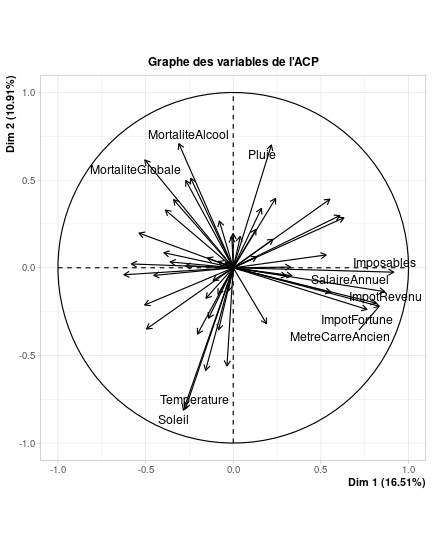
\includegraphics[width=0.3\linewidth]{images/ACP_var_12_contrib.png} & 
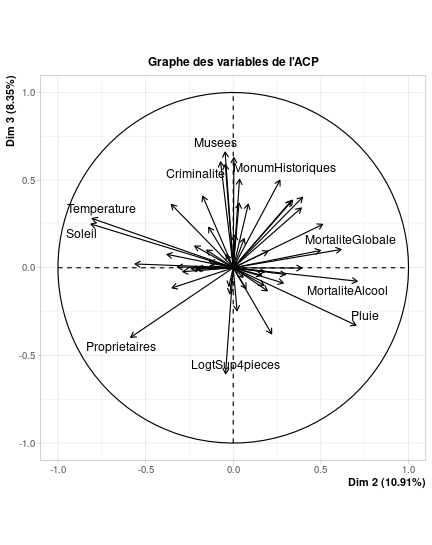
\includegraphics[width=0.3\linewidth]{images/ACP_var_23_contrib.png} & 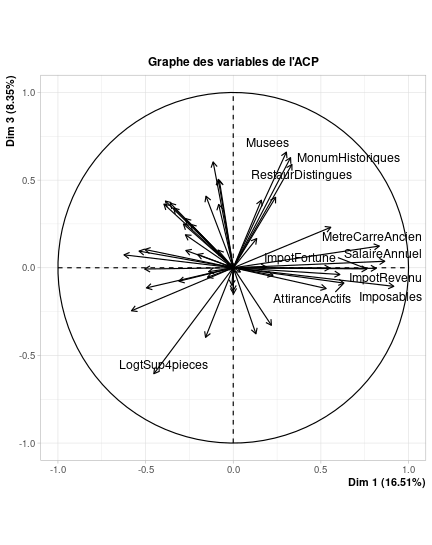
\includegraphics[width=0.3\linewidth]{images/ACP_var_13_contrib.png}• \\ 
\end{tabular} 
\end{center}

{\large \textbf{Axe 1}}

\begin{itemize}
	\item[$\bullet$] \textbf{Contribution}

	Tout d'abord, observons que $ \frac{1}{54}\approx 2\%$ ce qui nous 	pousse à ne considérer que les variables dont la contribution est très supérieure à $2\%$. On trouve alors : \emph{Imposables} (9,41\%), \emph{SalairesAnnuels} (8,38\%), \emph{MetreCarreAncien} (7,75\%), \emph{ImpotRevenu} (7,46\%) et \emph{ImpotFortune} (6,52\%). En additionnant, leur contribution on obtient : $39,52\%$ ce qui est très supérieur à $5\times 2\%=10\%$. Ce sont donc des variables économiques qui contribuent en une part importante à la fabrication de l'axe 1. On voit d'ailleurs sur le plan (1,2), ce groupe de variables allant dans la même direction.

	\item[$\bullet$] \textbf{Originalité : COS2}
	
	On retrouve ici, les mêmes variables que précédemment et dont l'originalité est principalement décrite par l'axe 1 : \emph{Imposables} (0,84), \emph{SalairesAnnuels} (0,75), \emph{ImpotFortune} (0,66), \emph{MetreCarreAncien} (0,65). \\
	
On peut en conclure que cet axe 1 décrit des marqueurs de richesse.
	
\end{itemize}

\bigskip

{\large \textbf{Axe 2}}

\begin{itemize}
\item[$\bullet$] \textbf{Contribution}
Parmi les variables dont la contribution est très supérieure à $2\%$, il y a : \emph{Soleil} (11,20\%), \emph{Température} (11,01\%), \emph{MortaliteAlcool} (8,50\%), \emph{Pluie} (8,33\%) et \emph{MortaliteGlobale} (6,43\%). De manière cumulée, on obtient 45,47\%. Sur la représentation du plan (1,2), on voit ces variables s'opposer : \emph{Soleil} et \emph{Température} d'un côté, les trois restantes de l'autre.  

\item[$\bullet$] \textbf{Originalité : COS2}
L'originalité des variables \emph{Soleil} et \emph{Temperature} est capturée à hauteur de $0,66$ et $0,65$ par l'axe 2. Si on leur ajoute leurs valeurs sur les axes 1 et 3, on trouve \emph{Soleil} : 0,8 et \emph{Temperature} : 0,8 aussi. Pour la \emph{MortaliteAlcool}, on a $0,50$ sur l'axe 2 et $0,61$ si l'on considère les trois axes. De même, le COS2 de la mortalité globale est de $0,38$ le long de l'axe 2 et $0,64$ si l'on considère les 3 axes. Enfin pour la pluie, on trouve $0,49$ sur l'axe 2 et $0,65$ pour les 3 axes.

Ici on commence à avoir une idée de ce que semble représenter cet axe : une opposition entre le Nord et le Sud de la  France. L'étude ultérieure des individus nous permettra d'en dire  certainement plus.

\end{itemize} 

\bigskip

{\large \textbf{Axe 3}}

\begin{itemize}
\item[$\bullet$] \textbf{Contribution}

Voici un tableau des variables les plus contributives à la fabrication de l'axe 3 : 

\begin{tabular}{|l|c|c|c|c|c|c|}
\hline 
Variables & Musées  & MonumentHistorique & LogtSup4Pieces & Criminalite & RestauDistingues & Total \\ 
\hline 
Contribution & 9,65 & 8,15 & 8,10 & 8,08 & 7,70 & 41,68 \\ 
\hline 
\end{tabular} 

\item[$\bullet$] \textbf{Originalité : COS2}

Pour ce qui est de l'originalité, on ne retrouve rien de très significatif. Celle-ci semble être diluée dans davantage d'axes que les 3 considérés. 

\begin{tabular}{|l|c|c|c|c|c|}
\hline 
Variables & Musées  & MonumentHistorique & LogtSup4Pieces & Criminalite & RestauDistingues \\ 
\hline 
Originalité sur l'axe 3 & 0,44 & 0,39 & 0,37 & 0,36 & 0,35  \\ 
\hline
Originalité sur les 3 axes & 0,53 & 0,5 & 0,58 & 0,38 & 0,46  \\ 
\hline  
\end{tabular} 

Si l'on observe les plans (2,3) et (1,3), on peut voir un faisceau entre des variables culturelles \emph{Musées}, \emph{MonumentHistorique} et \emph{RestauDistingues}, la variable \emph{LogtSup4Pieces} étant elle négativement corrélée aux trois précédentes. L'originalité de la variable criminalité n'étant finalement pas suffisamment décrite par l'axe 3, on peut supposer que l'axe 3 reflète plutôt une tendance culturelle et qui va opposer grandes et petites villes. 
\end{itemize}

\subsection{Etude des individus}

Voici le graphique du plan (1,2) avec les 10 individus les plus contributifs : 

\centerline{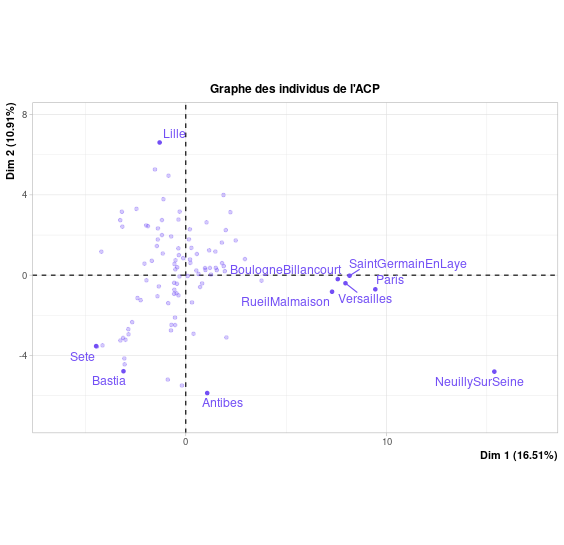
\includegraphics[width=0.5\linewidth]{images/ACP_ind_12_contrib}} 

Pour ce qui concerne la contribution, nous comparerons les valeurs avec la contribution moyenne $\frac{1}{100}=0,01$.

\bigskip

{\large \textbf{Axe 1}}

\begin{itemize}
\item[$\bullet$] \textbf{Contribution} 
Six villes ont une contribution forte pour l'axe 1 dont une plus particulièrement : 

\begin{center}
\begin{tabular}{|l|*{7}{m{1.7cm}|}}
\hline 
Individus & Neuilly-Sur-Seine  & Paris & Saint-Germain-en-Layes & Versailles & Boulogne-Billancourt & Rueil-Malmaison & Total \\ 
\hline 
Contribution & 26,51 & 10,0 & 7,46 & 7,10 & 6,43 &  5,96 & 63,46 \\ 
\hline 
\end{tabular}
\end{center}

La contribution de ces six villes est très largement supérieure à la contribution moyenne de $6\%$.

\item[$\bullet$] \textbf{Originalité : COS2}

Les villes dont l'originalité est largement supportée par l'axe 1 sont les mêmes que précédemment à l'exception notable de Paris : 

\begin{center}
\begin{tabular}{|l|*{6}{m{2cm}|}}
\hline 
Individus & Versailles  & Saint-Germain-en-Layes & Neuilly-Sur-Seine  & Boulogne-Billancourt &  Rueil-Malmaison \\ 
\hline 
Originalité & 0,73 & 0,67 & 0,65 & 0,61 & 0,57\\ 
\hline 
\end{tabular}
\end{center} 

L'originalité de Paris le long de cet axe est seulement de 0,25. Ceci semble indiqué que Paris n'est pas seulement originale par sa dimension économique mais que son originalité est multiple. 
\end{itemize}

Ce que l'on peut conclure de cette étude de l'axe 1, c'est que ce dernier représente effectivement des variables économiques et que quelques villes de l'Ouest parisien contribue fortement à son orientation. Si l'on met côte à côte la plan (1,2) du graphe de l'ACP des variables et celui des individus, on remarque évidemment une direction similaire entre les variables étudiées et les villes contributives.

\bigskip

{\large \textbf{Axe 2}}

\begin{itemize}
\item[$\bullet$] \textbf{Contribution}

Les principales contributions à la construction de l'axe 2 sont données par 6 villes : \emph{Lille} (7,42\%), \emph{Antibes} (5,85\%), \emph{Cannes} (5,13\%), \emph{Valenciennes} (4,71\%), Nice (4,60\%) et Saint-Denis (4,17\%). En additionnant leur contribution, on obtient 31,88\%. 

\item[$\bullet$] \textbf{Originalité : COS2}

Les cnq villes dont l'originalité est décrite partiellement par cet axe 2 sont : \emph{Lille} (0,47), \emph{Antibes} (0,44), \emph{Troyes} (0,42), \emph{Nice} (0,40) et \emph{Valenciennes} (0,38).
\end{itemize}

De cet axe 2 se dégage un axe Nord-Sud. Au Nord, des villes pluvieuses avec une mortalité globale supérieure et au Sud des villes chaudes et ensoleillées.

L'édition du plan (2,3) nous montre un regroupement de villes du Sud :

\centerline{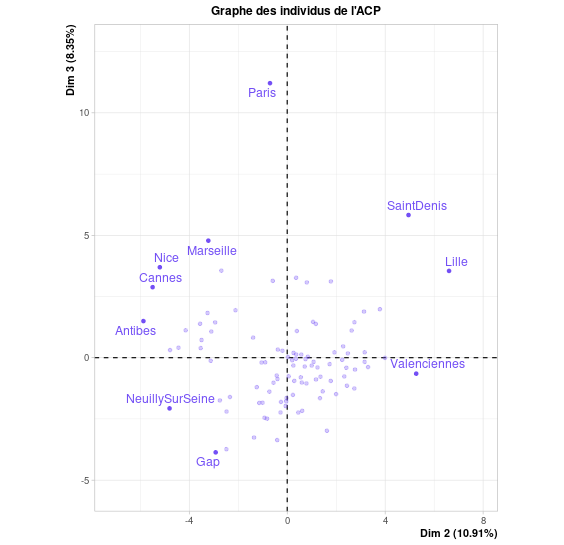
\includegraphics[width=0.5\linewidth]{images/ACP_ind_23_contrib}} 

Ce regroupement se trouve être justement dans la même direction que celui des variables \emph{Soleil} et \emph{Temperatures}.

\bigskip

{\large \textbf{Axe 3}}

Voici le plan (1,3) des individus : 

\centerline{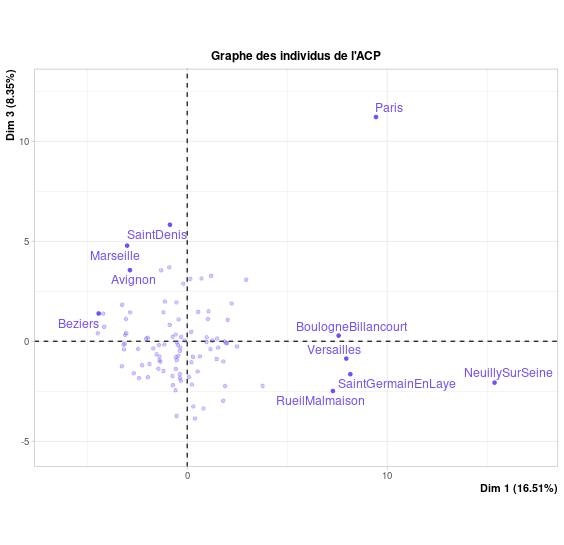
\includegraphics[width=0.5\linewidth]{images/ACP_ind_13_contrib}} 

\begin{itemize}
\item[$\bullet$] \textbf{Contribution}

On trouve ici quelques contributeurs importants et notamment une ville singulière \emph{Paris} contribuant à hauteur de $27,86\%$. Les deux autres villes sont \emph{Saint-Denis} (7,53\%) et Marseille (5,06\%). Dans une moindre mesure : \emph{Gap} (3,31\%) et \emph{Cholet} (3,09\%) contribue à la construction de cet axe.

\item[$\bullet$] \textbf{Originalité COS2}

Aucune ville ne semble être majoritairement décrite par cet axe 3. Toutefois on peut remarquer un fait notable. Nous avions dit que Paris, bien que contributeur de l'axe 1, ne voyait pas son originalité y être décrite. Paris se trouve être plus original selon cet axe 3 (0,35) auquel il participe grandement à sa construction. Les villes contributrices tirent une part de leur originalité de cet axe : \emph{Marseille} (0,29),  \emph{Cholet} (0,28) \emph{Saint-Denis} (0,26) et Gap (0,22).

Enfin \emph{La-Roche-Sur-Yon} a un COS2 égale à 0,31.
\end{itemize}

En superposant les plans où se trouvent l'axe 3, on remarque évidemment que les variables contributives à sa construction la position de Paris ne sont pas étrangères. La direction et la même et cela est du au fait que Paris a une contribution majeure à cet axe. Elle en tire d'ailleurs son originalité principale. Cet axe semble être celui des marqueurs culturels. 

\subsection{Conclusion}

On retrouve dans cet ACP, les résultats obtenus dans le TP2 où le dendogramme donnait une impression visuelle de former 3 classes : 

\centerline{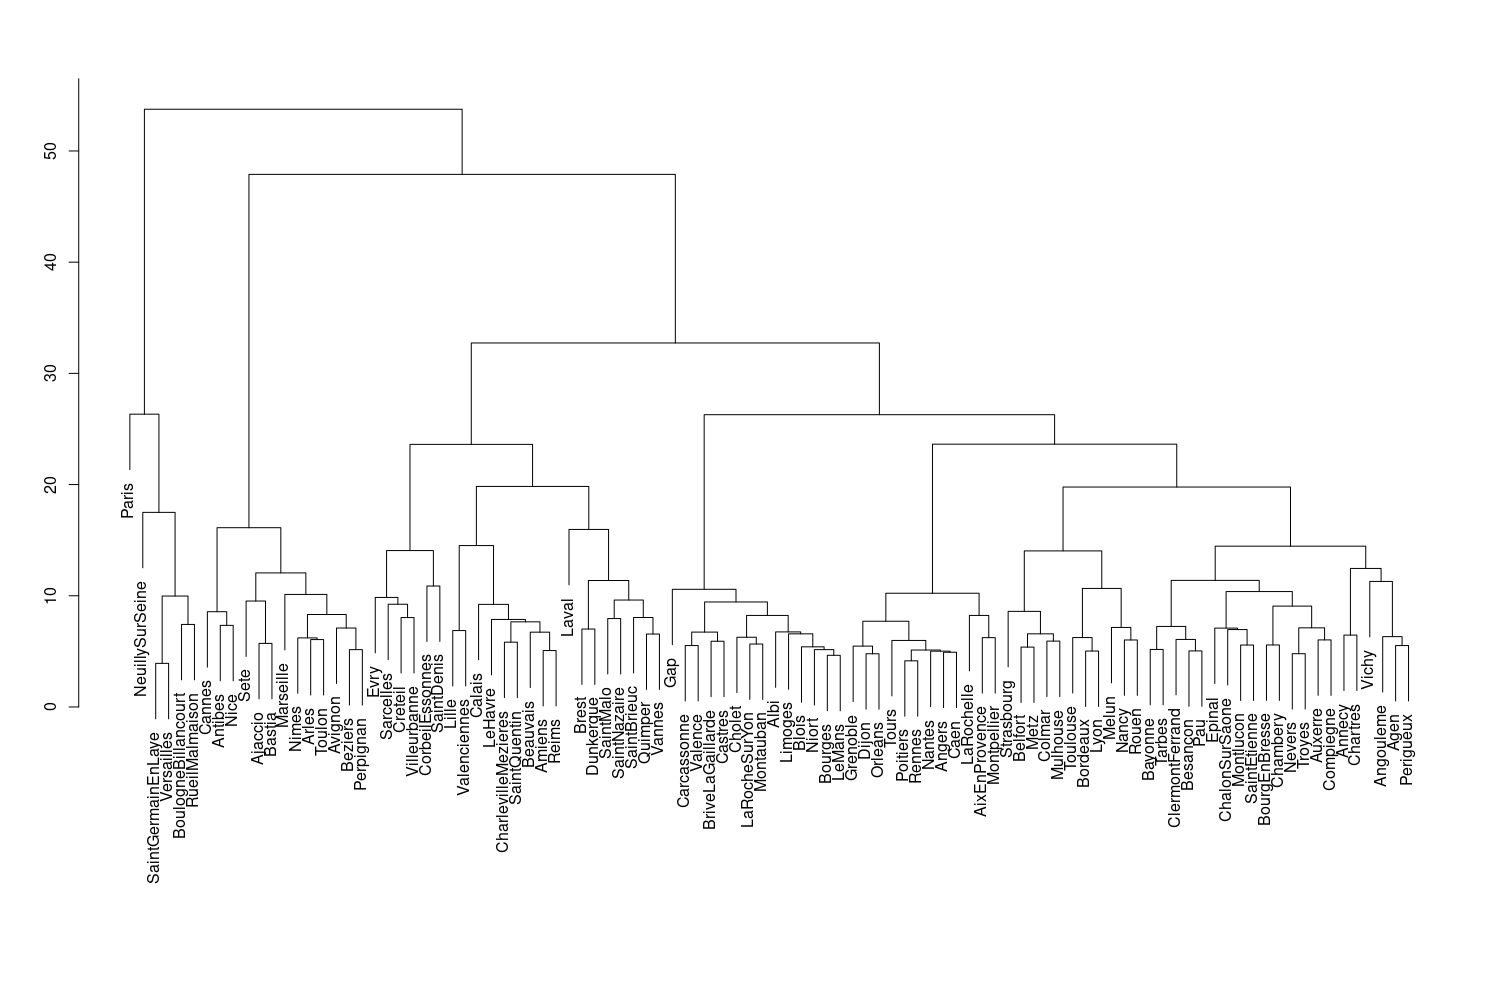
\includegraphics[width=0.5\linewidth]{images/Dendo}} 

On retrouve dans cette ACP, 3 axes principaux : 
\begin{itemize}
\item[$\bullet$] \textbf{Axe 1 :} axe à dominante économique avec de gros contributeurs se caractérisant par une position géographique bien particulière : l'Ouest parisien. 
\item[$\bullet$]  \textbf{Axe 2 :} celui-ci oppose le Sud ensoleillé et chaud au Nord pluvieux dont certaines variables au caractère plus morbide sont contributrices. 
\item[$\bullet$] \textbf{Axe 3 :} Cette fois ci c'est la culture qui se distingue mais la culture parisienne. En effet, il s'agit d'un contributeur majeur isolé à sa fabrication.  
\end{itemize}

\section{ACP de rang sur l'ensemble des variables}

Après avoir obtenu la matrice des rangs, nous lançons l'ACP avec Factoshiny. 

	\subsection{Etude de la variance cumulée}
	
Nous nous intéressons, comme pour l'ACP normée, aux valeurs propres dont voici le graphique :
	
\centerline{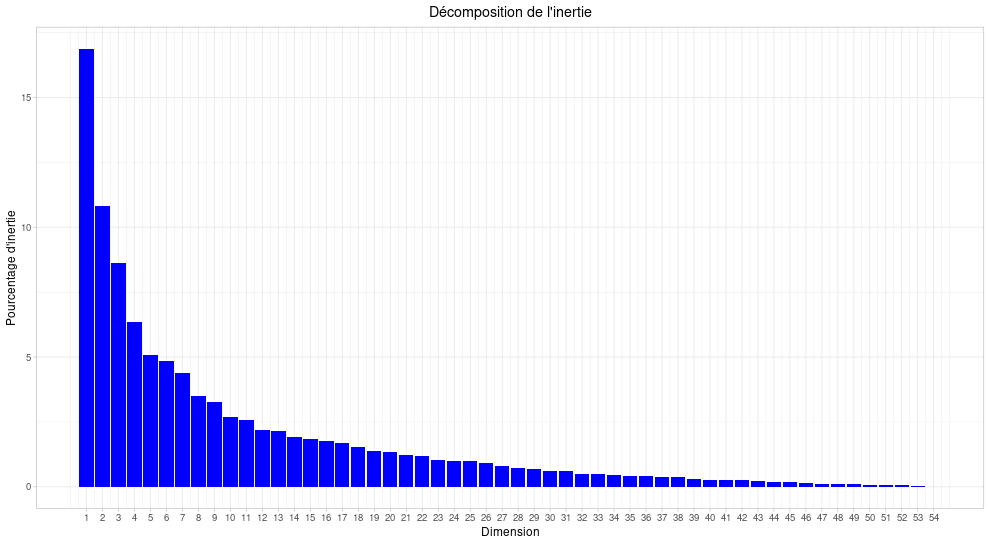
\includegraphics[width=0.8\linewidth]{images/ACPR_vp}}

et le tableau de valeurs :

\begin{center}
 \begin{tabular}{|l|*{8}{>{\centering\arraybackslash}p{1cm}|}}
 \hline 
 \rule[-1ex]{0pt}{2.5ex} Valeurs propres & Dim.1  & Dim.2 &  Dim.3 &  Dim.4 &  Dim.5 &  Dim.6 &  Dim.7 & Dim.8\\ 
 \hline 
 \rule[-1ex]{0pt}{2.5ex}  Variance & 9.110 &   4.511 &  4.662 &  3.422 &  2.752 &  2.616  & 2.358 &  1.879\\
 \hline 
 \rule[-1ex]{0pt}{2.5ex} 
$\%$ of var. &  16.871 & 10.825 &  8.634 &  6.338 &  5.096 &  4.844  & 4.366 &  3.480 \\
 \hline 
 \rule[-1ex]{0pt}{2.5ex} 
Cumulative $\%$ of var. & 16.871 & 27.696 & 36.330 & 42.668 & 47.764 & 52.608 & 56.974 & 60.455 \\
\hline
\end{tabular}
\end{center}

On a un décrochement entre la 4-ème et la 5-ème valeur ce qui nous pousse à nous intéresser aux quatre premiers axes. C'est déjà une différence avec l'ACP normée. 

\subsection{Etude des différents plans}

{\large \textbf{Plan (1,2)}}

Côte à côte voici les graphiques des individus et celui des variables avec les 25 plus gros contributeurs pour les individus et les 10 plus gros contributeurs pour les variables : 

\centerline{\begin{tabular}{ccc}
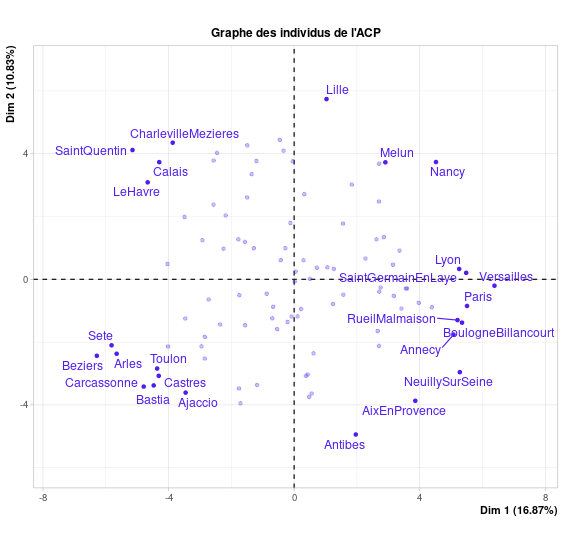
\includegraphics[width=0.55\linewidth]{images/ACPR_ind_12} & 
&
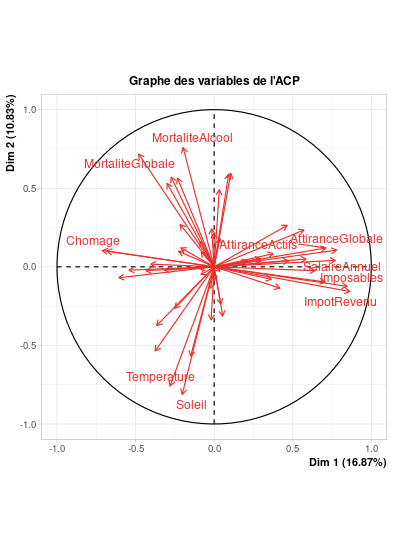
\includegraphics[width=0.40\linewidth]{images/ACPR_var_12}
\end{tabular}}

On retrouve le même faisceau des variables de richesse que sur l'ACP normée, auxquelles viennent se rajouter \emph{AtiranceActifs} et \emph{AttiranceGlobale}. Ces variables sont à mettre en opposition à la variable chômage qui décrit plus la pauvreté. Dans la même direction se trouvent les villes trouvées lors de l'ACP normée, celle de l'Ouest parisien. Des villes réputées riches comme \emph{Lyon}, \emph{Annecy} ou bien \emph{Aix-en-Provence} viennent compléter la liste.


\textbf{Tableau des variables les plus contributrices pour l'axe 1 :}
\begin{center}
\begin{tabular}{|c|c|c|c||c|c|c|c|}
\multicolumn{4}{c}{Côté -} & \multicolumn{4}{c}{Côté +}\\
\hline 
Variables & Coordonnées & CTR & COS2 & COS2 & CTR & Coordonnées & Variables \\ 
\hline 
Chômage & $-0.71$ & $5.55$ & $0.51$ & $0.75$ & $8.19$ & $0.86$ & ImpotRevenu  \\ 
\hline 
 &  &  &  & $0.71$ & $7.85$ & $0.85$ & Imposables\\ 
\hline 
 &  &  &  & $0.61$ & $6.67$ & $0.78$ & AttiranceGlobale \\ 
\hline 
\end{tabular} 
\end{center}

\bigskip

\textbf{Tableau des individus les plus contributeurs pour l'axe 1 :}
\begin{center}
\begin{tabular}{|c|c|c|c||c|c|c|c|}
\multicolumn{4}{c}{Côté -} & \multicolumn{4}{c}{Côté +}\\
\hline 
Villes & Coordonnées & CTR & COS2 & COS2 & CTR & Coordonnées & Villes \\ 
\hline 
Beziers & $-6.28$ & $4.33$ & $0.57$ & $0.58$ & $4.47$ & $6.38$ & Versailles \\ 
\hline 
Sète & $-5.81$  & $3.71$ & 0.41 & $0.44$ & $3.33$ & $5.51$ & Paris\\ 
\hline 
 &  &  &  & $0.40$ & $3.30$ & $5.48$ & Saint-Germain-En-Laye \\ 
\hline 
\end{tabular} 
\end{center}

Sur cet axe 1, il y a plusieurs points contributifs, mais peu sont illustratifs car seuls les COS2 de \emph{ImpotRevenu} et \emph{Imposables} sont importants.

\bigskip

L'axe 2 met en opposition des villes du Sud et du Nord avec deux groupes bien distincts. Ceci correspond à une opposition entre les variables \emph{Température}, \emph{Soleil} et les variables \emph{MortaliteAlcool} et \emph{MortaliteGlobale}. Ceci est clairement visible sur les deux tableaux suivants :

\textbf{Tableau des variables les plus contributrices pour l'axe 2 :}
\begin{center}
\begin{tabular}{|c|c|c|c||c|c|c|c|}
\multicolumn{4}{c}{Côté -} & \multicolumn{4}{c}{Côté +}\\
\hline 
Variables & Coordonnées & CTR & COS2 & COS2 & CTR & Coordonnées & Variables \\ 
\hline 
Soleil & $-0.81$ & $11.27$ & $0.66$  & $0.58$  & $9.85$ & $0.76$ & MortaliteAlcool  \\ 
\hline 
 Temperature& $-0.76$ & $9.83$ & $0.57$ & $0.51$ & $8.80$ &  $0.72$ & MortaliteGlobale\\ 
\hline 
Vieillissement & $-0.57$  & $5.52$ & $0.32$ &  &  & &  \\ 
\hline 
\end{tabular} 
\end{center}

\bigskip

\textbf{Tableau des individus les plus contributeurs pour l'axe 2 :}
\begin{center}
\begin{tabular}{|c|c|c|c||c|c|c|c|}
\multicolumn{4}{c}{Côté -} & \multicolumn{4}{c}{Côté +}\\
\hline 
Villes & Coordonnées & CTR & COS2 & COS2 & CTR & Coordonnées & Villes \\ 
\hline 
Antibes & $-4.94$ & $4.18$ & $0.33$ & $0.52$ & $5.64$ & $5.74$ & Lille \\ 
\hline 
 &   &  &  & $0.33$ & $3.38$ & $4.44$ & Valenciennes\\ 
\hline 
 &  &  &  & $0.22$ & $3.12$ & $4.27$ & Saint-Denis\\ 
\hline 
\end{tabular} 
\end{center}


{\large \textbf{Plan (3,4)}}

\centerline{\begin{tabular}{ccc}
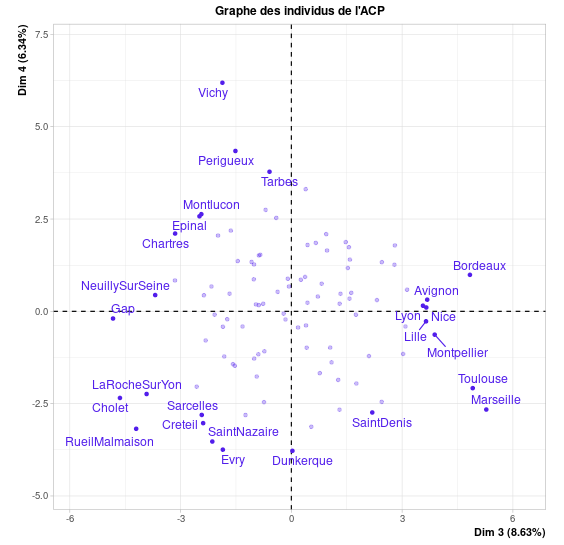
\includegraphics[width=0.55\linewidth]{images/ACPR_ind_34} & 
&
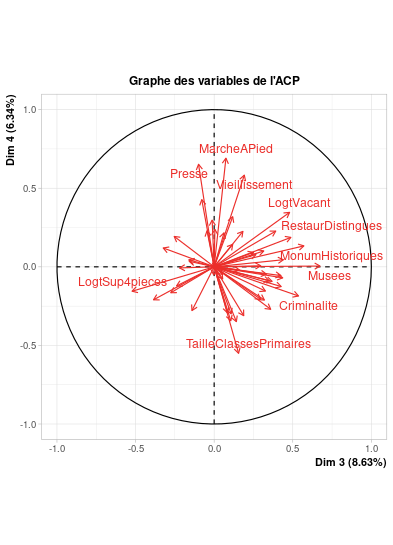
\includegraphics[width=0.40\linewidth]{images/ACPR_var_34}
\end{tabular}}

En observant ces deux graphiques, il ressort que les variables les mieux représentées pour l'axe 3 sur le plan sont \emph{Musées}, \emph{MonumHistoriques}, \emph{Criminalité} et \emph{RestauDistingue}. Ces variables sont corrélées négativement à \emph{LogtSup4Pieces}. En regardant de plus près les individus contributeurs, on trouve des grandes villes françaises à droite qui font la part belle à la culture mais où la criminalité est importante. Par criminalité, il faut entendre le nombre d'infractions et délits commis. Les infractions relatives au code de la route y sont forts nombreuses dans les grandes villes.

\textbf{Tableau des variables les plus contributrices pour l'axe 3 :}
\begin{center}
\begin{tabular}{|c|c|c|c||c|c|c|c|}
\multicolumn{4}{c}{Côté -} & \multicolumn{4}{c}{Côté +}\\
\hline 
Variables & Coordonnées & CTR & COS2 & COS2 & CTR & Coordonnées & Variables \\ 
\hline 
LogtSup4Pieces & $-0.52$ & $5.85$ & $0.27$  & $0.45$  & $9.72$ & $0.67$ & Musées  \\ 
\hline 
&  &  &  & $0.33$ & $6.99$ &  $0.57$ &  MonumHistoriques\\ 
\hline 
&  &  &  & $0.29$ & $6.18$ & $0.54$ & Criminalité \\ 
\hline 
&  &  &  & $0.32$ & $5.11$ & $0.49$ & RestauDistingues \\ 
\hline
\end{tabular} 
\end{center}

\bigskip

\textbf{Tableau des individus les plus contributeurs pour l'axe 3 :}
\begin{center}
\begin{tabular}{|c|c|c|c||c|c|c|c|}
\multicolumn{4}{c}{Côté -} & \multicolumn{4}{c}{Côté +}\\
\hline 
Villes & Coordonnées & CTR & COS2 & COS2 & CTR & Coordonnées & Villes \\ 
\hline 
Gap & $-4.83$ & $5$ & $0.33$ & $0.44$ & $5.98$ & $5.28$ & Marseille\\
\hline
 Cholet & $-4.64$  & $4.62$  & $0.33$ & $0.43$ & $5.17$ & $4.91$ & Toulouse\\ 
\hline 
 &  &  &  & $0.40$ & $5.02$ & $4.84$ & Bordeaux\\ 
\hline 
\end{tabular} 
\end{center}

La principale différence avec l'ACP normée c'est que l'on ne retrouve pas Paris sur cet axe alors qu'il en était le principal contributeur précédemment. Le fait de faire une ACP de rang à éliminer une grande partie de la singularité de Paris et les variables culturelles qui la décrivait. Ici les COS2 sont plutôt faibles et l'originalité des villes est partiellement mis en évidence ici.

\bigskip

Sur l'axe 4, trois variables ont une forte contribution : \emph{MarcheAPied} (13.95), \emph{Presse} (12.43) et \emph{Vieillissement} (9.94). Pour ce qui est des villes, deux sortent du lot \emph{Vichy} (11.20) et \emph{Tarbes} (4.17). L'originalité de Vichy est tirée à 50\% par ces variables et à 31\% pour Tarbes. Concernant les variables, \emph{MarcheaPied} tire 48\% de son originalité le long de cet axe, 43\% pour \emph{Presse} et 34\% pour \emph{Vieillissement}. 

\bigskip

Ces trois variables semblent décrire des variables liées à une population de retraités. Il faudrait regarder plus en détails les villes concernées pour en avoir le c\oe ur net. 

\subsection{Conclusion}

Cette ACP de rang a permis de dégager d'autres résultats. En effet sur l'axe 1, Neuilly-Sur-Seine était un individu très singulier de part sa contribution disproportionné. L'ACP de rang a permis de gommer cette singularité. De même, l'axe 3 s'est trouvé modifier car la contribution de Paris a été amoindri permettant de faire émerger d'autres villes où la culture était bien présente. 


\section{ACP normé pour les différents thèmes}

\subsection{Thème Economie} 
Voici le graphique des valeurs propres :

\centerline{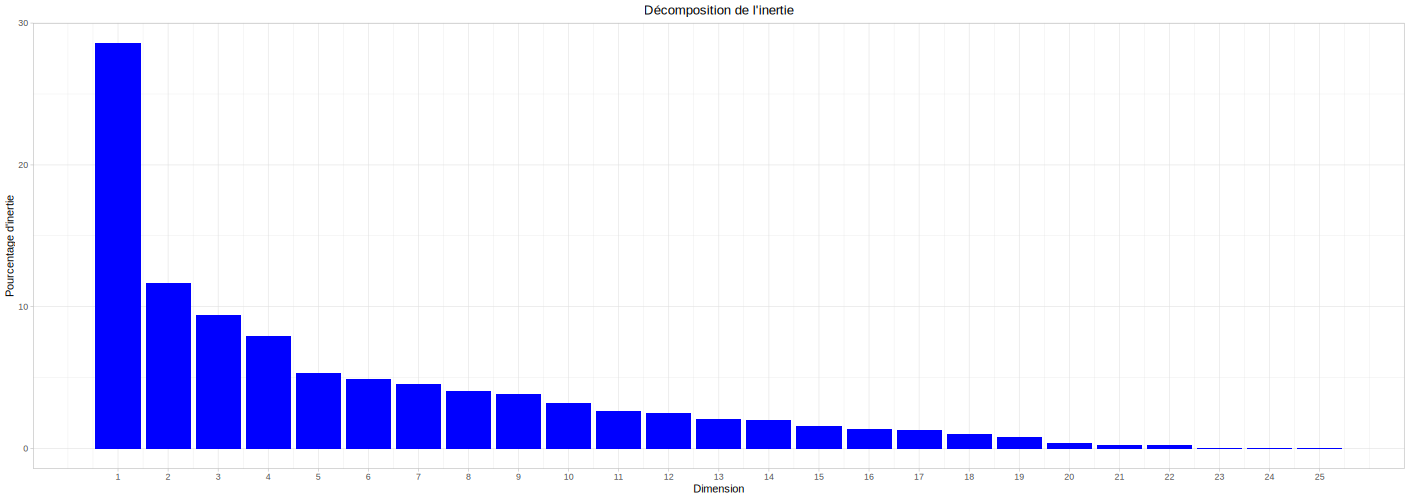
\includegraphics[width=0.8\linewidth]{images/VP1}}
n'ayant de décrochement claire qu'aprés la 4em valeur propre,
On se restreindra a 2 axes qui permettrons d'explorer 40,25\% de la variance totale pour le theme economie,

\centerline{\begin{tabular}{ccc}
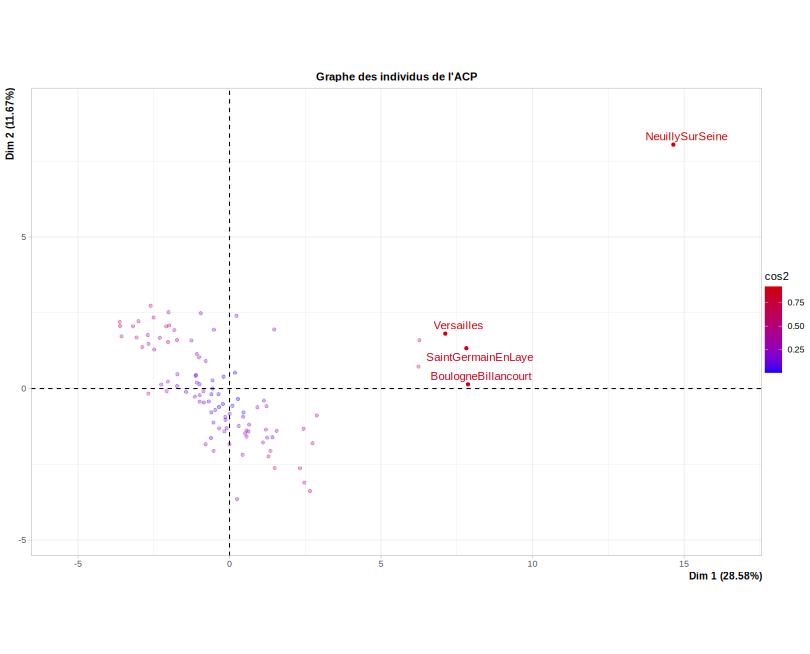
\includegraphics[width=0.55\linewidth]{images/I_1_0,85} &
&
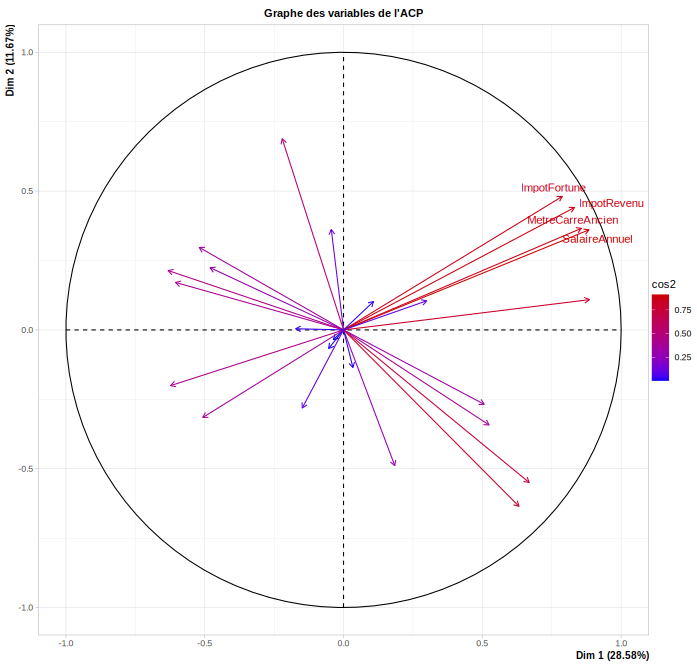
\includegraphics[width=0.40\linewidth]{images/V_1_0,85}
\end{tabular}}

Se limiter aux individus et variable les mieux représenté dans un premier temps \emph(cos2>0,85)\%
dégage un premier cluster "SalaireAnnuel", "ImpotRevenu", "ImpotFortune","MetreCarreAncien" portée par les villes de l'ouest parisien.\\
Ce plan est alors fortement déterminer par les indicateur du niveau de richesse de ces villes, c'est concidération qui nous sert de levier d'interprétation la suite :

\centerline{\begin{tabular}{ccc}
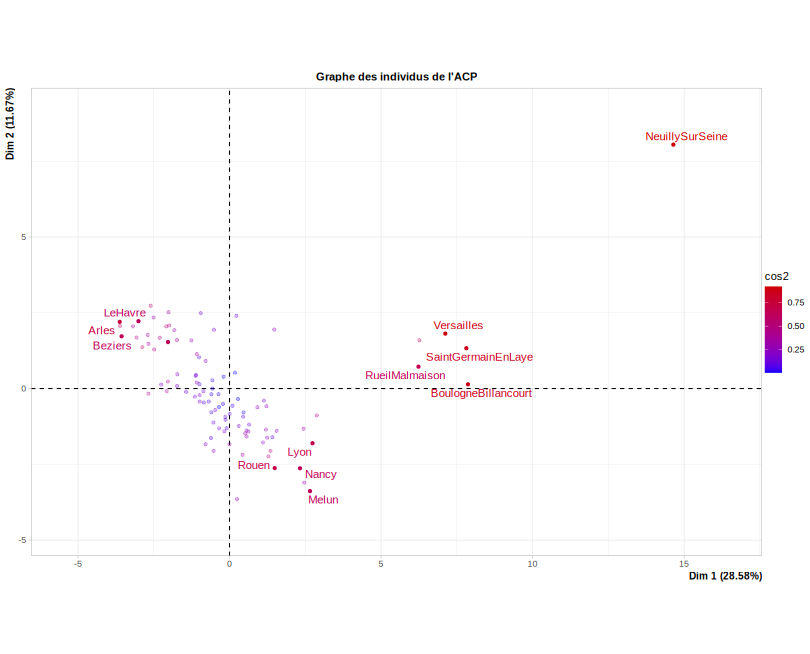
\includegraphics[width=0.55\linewidth]{images/I_1_0,6} &
&
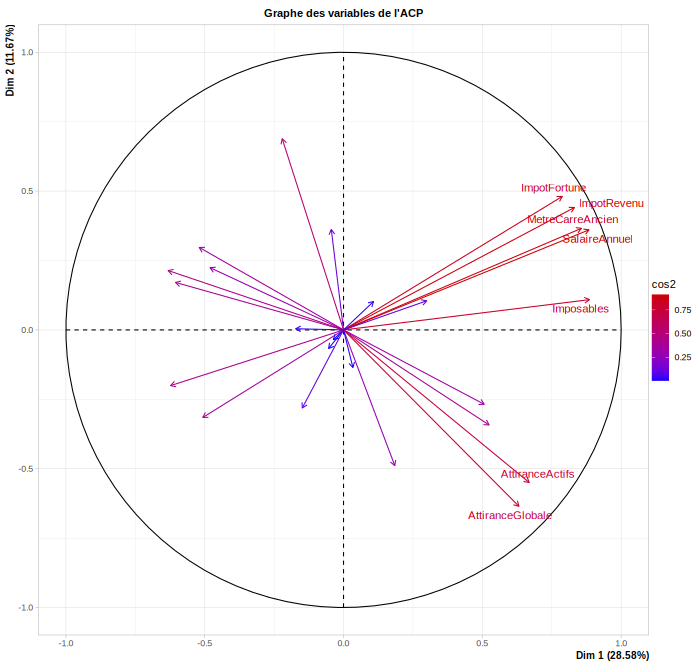
\includegraphics[width=0.40\linewidth]{images/V_1_0,6}
\end{tabular}}

En étant plus tolérant \emph(cos2>0,6)\% : un deuxieme cluster  "AttiranceGlobale", "AttiranceActifs" se détaches, et deux nouveau groupes s'opposant apparaissent :\\
D'une part : Lyon,Nancy,Melun et Rouen, qui on permis la détermination de ce cluster par leur point commun (une fort valeur d'attirance Global et Actif) mais surtout leur différences communes : elles sont toutes loins derriere l'ouest parisien en niveau de richesse.\\
Notons que dans le tableau de donnée brut, le top 10 dans ces 2 catégorie est présque partager entre ce groupes et l'ouest parisien, ce qui renforce l'idée c'est cette grande différence qui a permis l'émergeance de se second groupement.\\
D'autre part : LeHavre, Arles Beziers, qui forme un groupe antagoniste au deux précédent (ces trois villes étant dans le bas du classement dans la plus part des indicateur en richesse et attirance)\\

L'émergence de ce dernier groupe éclaire et améliore nos premiers traveau sur ce jeux de donnée :\\
On retrouve l'intuition de notre premiere interprétation des 3 classes obtenue (lors du TP2) par la CAH du theme, la riche region parisienne occupé déja ça propre classe (3) et
Lyon,Nancy,Melun et Rouen étaient bien dans la même classe des "villes relativement attractive"(1)\\

Mais avec une meilleur comprehention ici entre ce qui fait les point communs de la classe 1 et 3 (une haute attirance Global/Actif)
et ce qui fait de la classe 2 (dont LeHavre, Arles, Beziers font paris) une classe si différentes des deux autres : sont faible niveau de richesse ET faible attirance Global/Actif\\

\subsection{Thème Risques}

Voici le graphique des valeurs propres :

\centerline{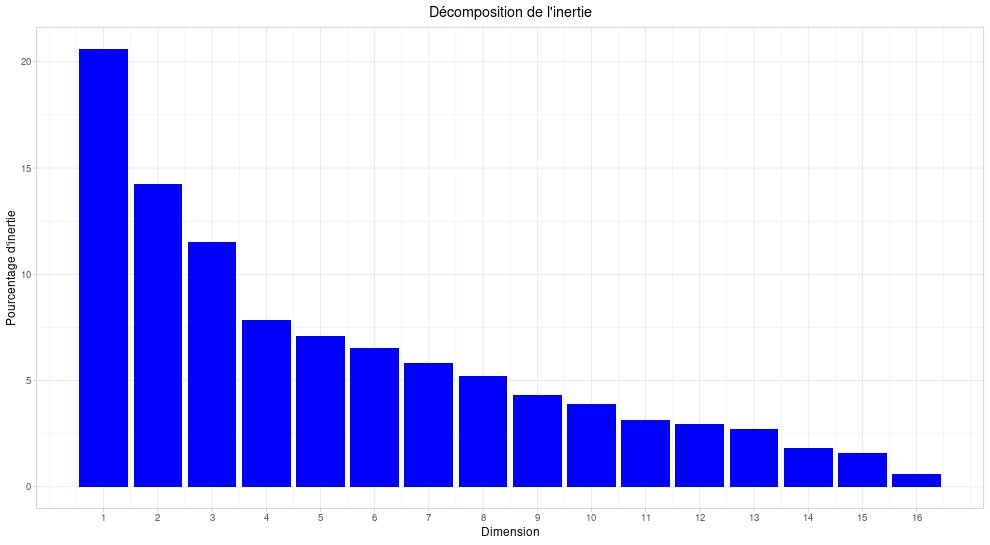
\includegraphics[width=0.8\linewidth]{images/ACP_ris_vp}}

On constate un décrochement entre la 3-ème et la 4-ème valeur propre. De plus, la variance cumulée sur les 3 premières valeurs propres est de 46,41\%. Nous considérerons 3 axes.

\bigskip

{\large \textbf{Plan (1,2)}}

\centerline{\begin{tabular}{ccc}
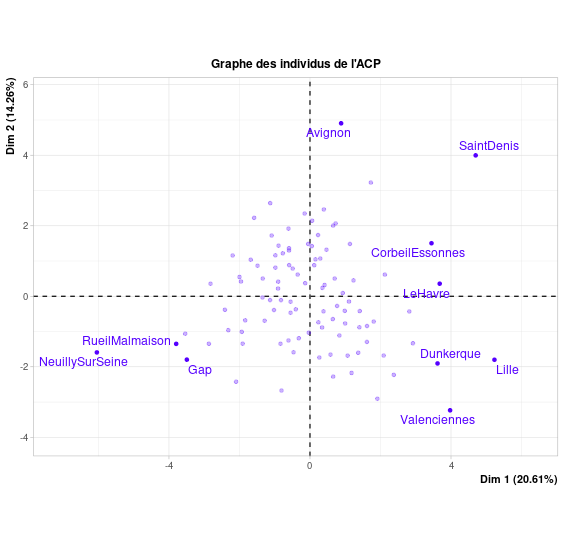
\includegraphics[width=0.55\linewidth]{images/ACP_ris_ind_12} &
&
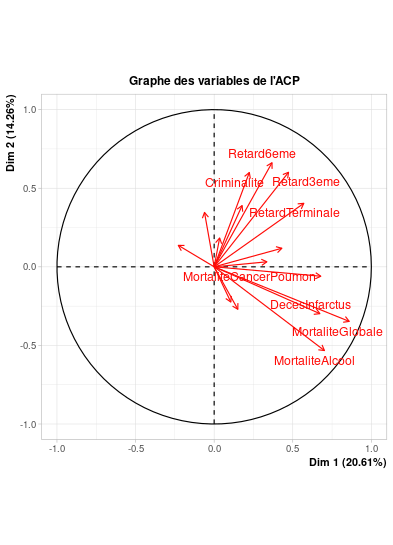
\includegraphics[width=0.40\linewidth]{images/ACP_ris_var_12}
\end{tabular}}

Voici les graphiques des individus avec les 10 plus gros contributeurs et celui des variables où sont indiquées les 8 variables les plus contributrices.

Du côté des variables, se dessinent deux faisceaux avec des thèmes propres. Un premier faisceau, qui nous parlent de mortalité : \emph{MortaliteGlobale} (CTR : 22,39\%), \emph{MortaliteAlcool} (14,92\%), \emph{MortaliteCancerPoumon} (13,95\%) et \emph{DecesInfarctus} (13,71\%). \emph{MortaliteGlobale} a d'ailleurs un COS2 assez élevé sur la première dimension : 0,74. Cette variable est donc assez bien corrélée avec la composante 1.\\

Trois villes  pointent de la même région pointent dans la même direction que les 4 variables précédemment citée : Lille (CTR : 8,30\% ;  COS2 : 0,67), Valenciennes (CTR1 : 4,79\% ; COS2 : 0,43) et Dunkerque (CTR1 : 3,97 ; COS2 : 0,41). Une autre ville est très contributrice au positionnement de l'axe 1, mais pointe dans la direction opposée : \emph{Neuilly-Sur-Seine} (CTR1 : 11,08\%). \\

Neuilly-Sur-Seine est aussi opposée au second faisceau de variables qui nous parle davantage de retard scolaire. Ces variables sont très contributrices au positionnement de l'axe 2. Il paraît malheureusement logique que ce retard scolaire dès la 6-ème (CTR2 : 19,21\%), soit perpétué en 3-ème (CTR2 : 15,85\%\%) puis en terminale (CTR2 : 7,15\%). La variables \emph{Ciminalite} participe aussi très fortement au positionnement de l'axe 2 avec une contribution de 15,78\%. Malgré de fortes contributions, l'étude des COS2 ne montre rien de très significatif \\

Du côté des individus, Avignon tire une bonne partie son originalité de cet axe avec un COS2 égale à 0,67. Elle pointe malheureusement dans la même direction que la criminalité et le retard scolaire.

\bigskip

{\large \textbf{Plan (2,3)}}

\centerline{\begin{tabular}{ccc}
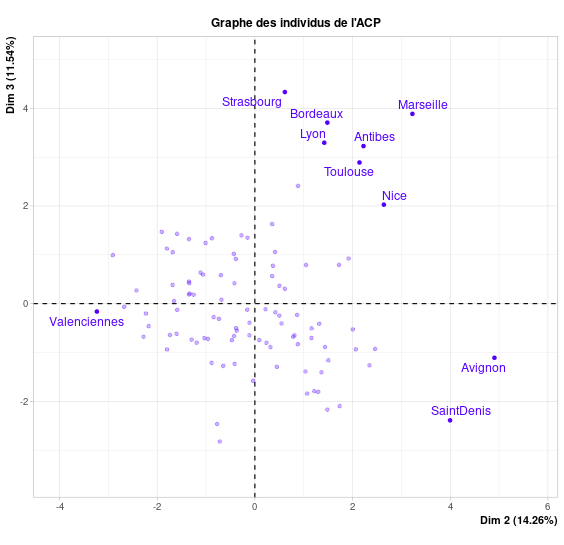
\includegraphics[width=0.55\linewidth]{images/ACP_ris_ind_23} &
&
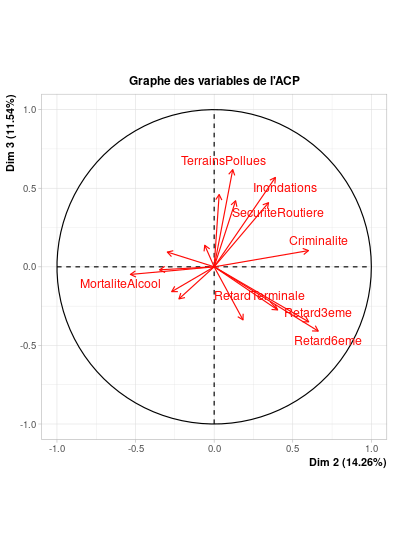
\includegraphics[width=0.40\linewidth]{images/ACP_ris_var_23}
\end{tabular}}

Sur ce plan, on distingue clairement un regroupement de plusieurs grandes villes de France qui contribuent au positionnement de l'axe 3 : \emph{Strasbourg} (CTR3 : 10,16\%) \emph{Marseille} (CTR3 :8,18\%), \emph{Bordeaux} (CTR3 : 7,44\%), Lyon (CTR3 : 5,88\%) et \emph{Toulouse} (CTR3 : 4,52\%). L'originalité de Bordeaux est d'ailleurs bien visible sur cet axe avec un COS2 de 0,69.\\

On retrouve parmi les variables les plus contributrices pointant dans la direction de ces villes : \emph{TerrainPollue} (CTR3 : 20,71\%), \emph{Inondations} (CTR3 : 17,50\%) et \emph{UsinesRisques : 11,45\%}. Toutefois il n'y pas de forte corrélation entre ces variables et l'axe 3, leur COS2 étant assez faible.

\bigskip

\subsection{Thème Culture}

On se restreindra a 2 axes qui permettrons d'explorer 63.80\% de la variance totale pour le theme culture

\centerline{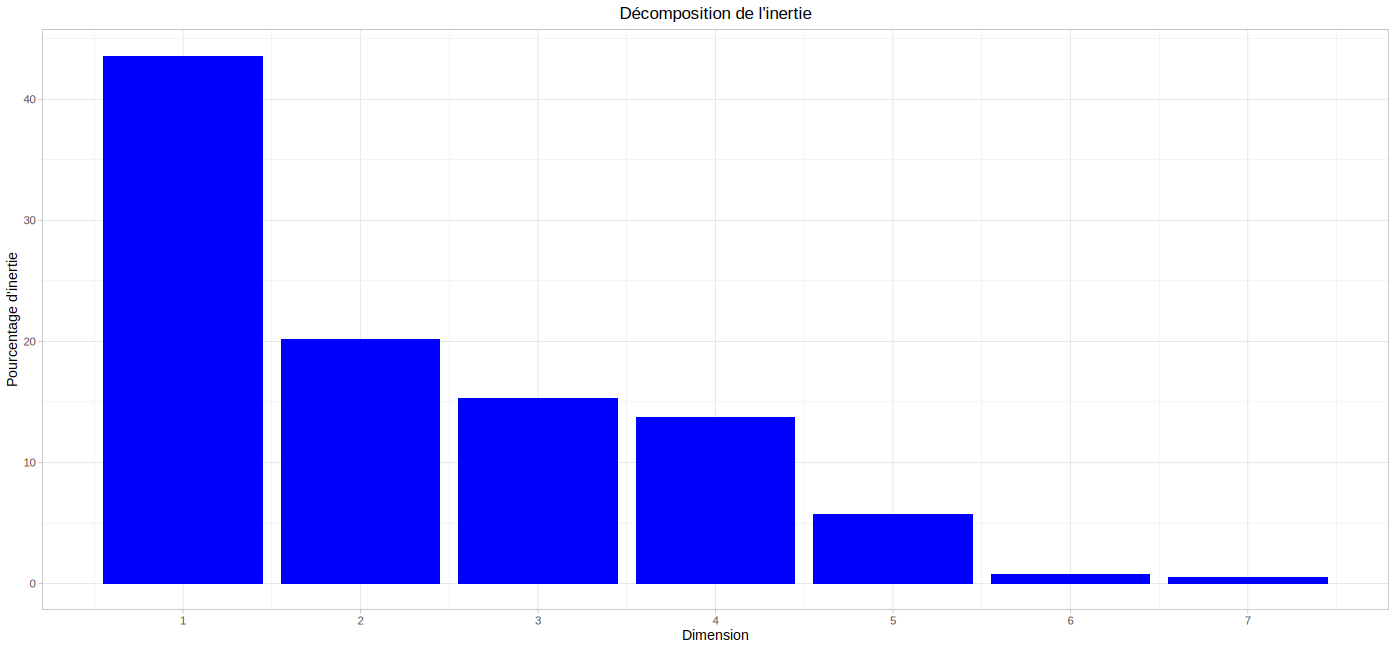
\includegraphics[width=0.5\linewidth]{images/VP3}}

\bigskip

\centerline{\begin{tabular}{ccc}
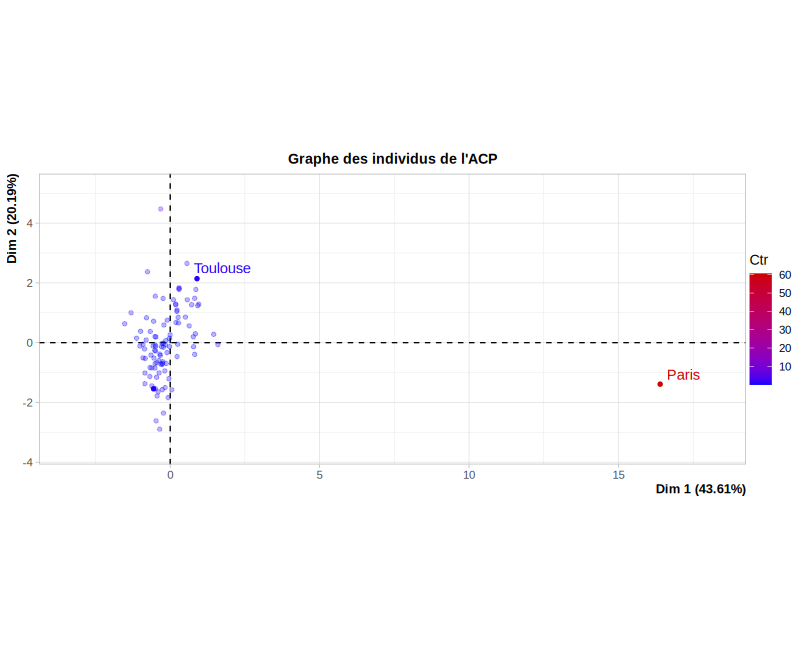
\includegraphics[width=0.55\linewidth]{images/I_3_0,9} &
&
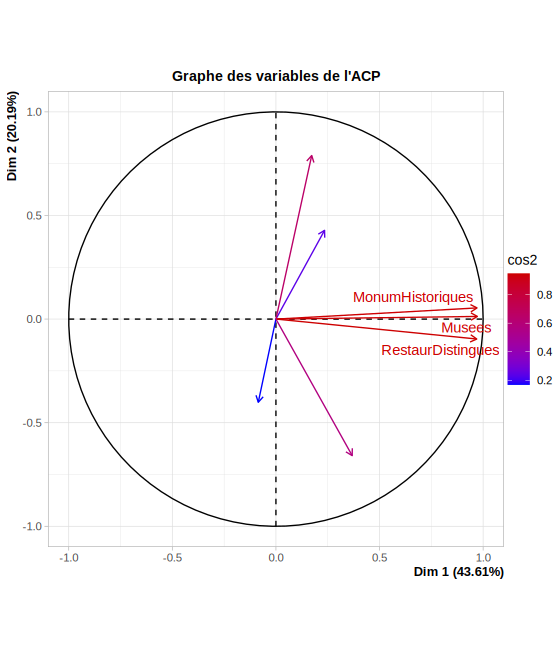
\includegraphics[width=0.30\linewidth]{images/V_3_0,9}
\end{tabular}}

Dans cette premiere ACP du theme culuture, la place énorme qu'occupe Paris dans la détermination du plan permet difficilement d'etudier l'etalement verticale qui se dessine en élargissant notre tolérance a \emph(cos2>0,5)\% :\\
\centerline{\begin{tabular}{ccc}
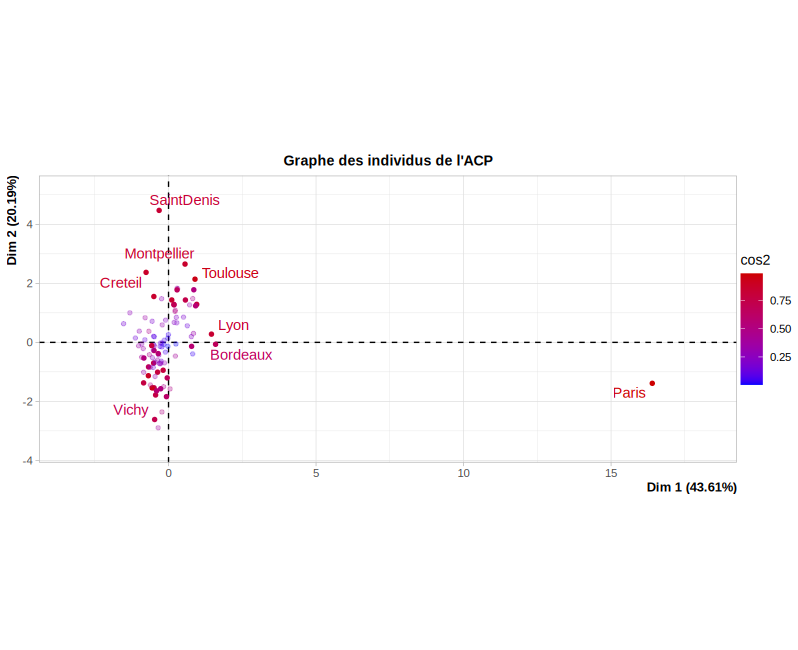
\includegraphics[width=0.55\linewidth]{images/I_3_0,5} &
&
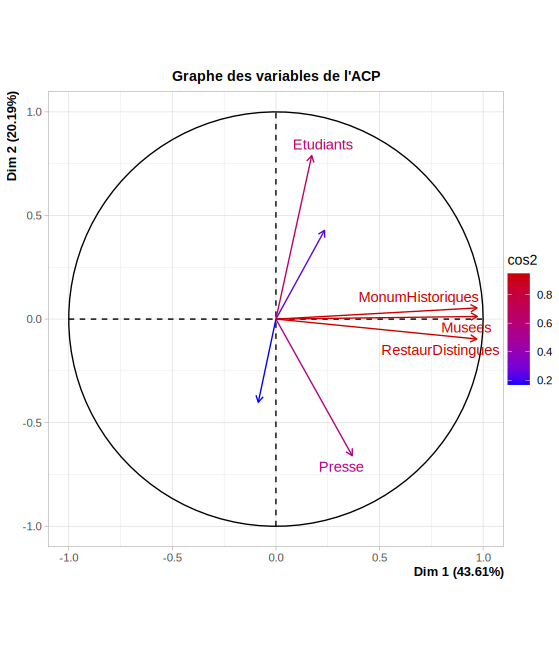
\includegraphics[width=0.30\linewidth]{images/V_3_0,5}
\end{tabular}}
Qui pourra étre mieux explorer dans l'ACP par rang.

	\subsection{Thème Nature}
	
Sur ce thème nous ne regarderons que les deux premiers axes. En effet ils capturent 73,75\% de l'information. On observe un décrochement entre la valeur propre 2 et la valeur propre 3 qui est de plus inférieure à 1.
	
\centerline{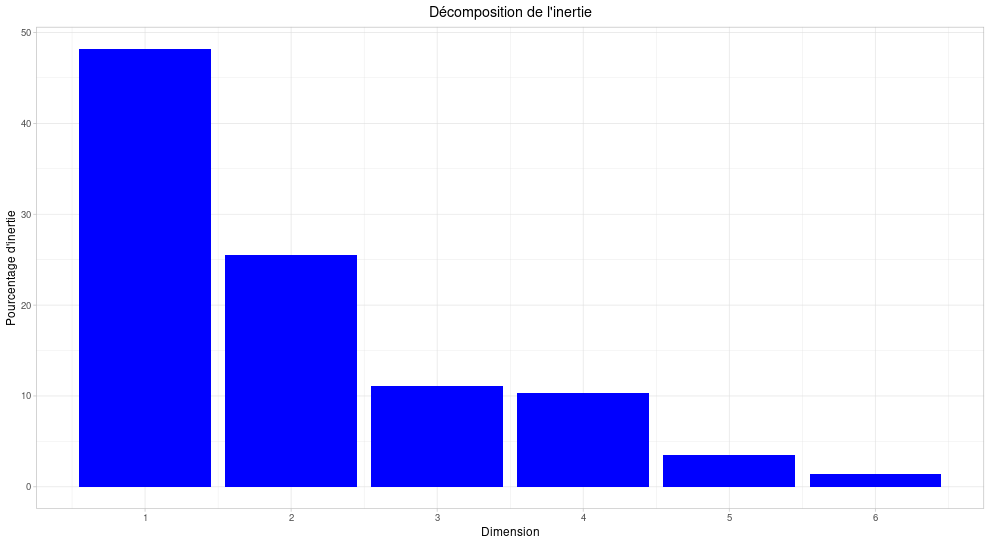
\includegraphics[width=0.8\linewidth]{images/ACP_nat_vp}}

\bigskip

{\large \textbf{Plan (1,2)}}

\centerline{\begin{tabular}{ccc}
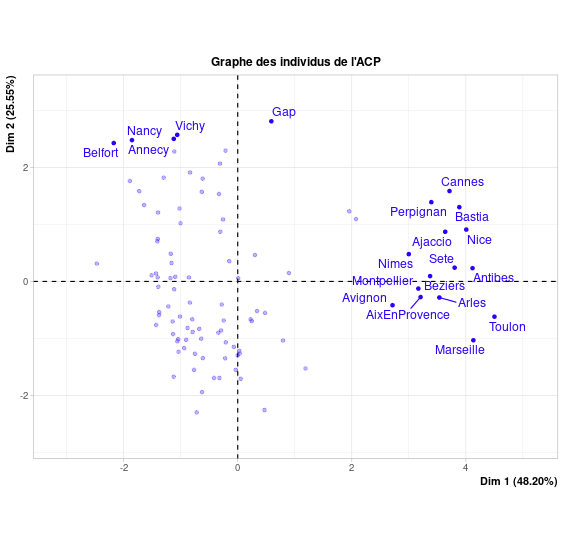
\includegraphics[width=0.55\linewidth]{images/ACP_nat_ind_12} & 
&
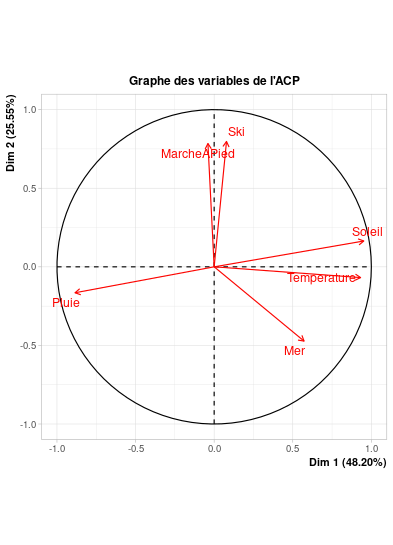
\includegraphics[width=0.40\linewidth]{images/ACP_nat_var_12}
\end{tabular}}

Ici l'étude est assez simple. On remarque 3 variables qui ont positionnées l'axe 1 : \emph{Soleil} (CTR : 31,33\%), \emph{Temperature} (CTR : 30,00\%) et \emph{Pluie} (CTR : 27,09\%). La variable \emph{Pluie} est logiquement anti-corrélée aux deux autres. Ces trois variables sont très corrélées avec cet axe. Leur COS2 est respectivement de 0,91 ; 0,87 et 0,78.\\

Sur le plan des individus, on voit un grand groupe de villes du Sud de la France dans la même direction que les variables \emph{Soleil} et \emph{Température}. On peut citer par exemple : \emph{Toulon} (CTR1 : 7\% ; COS2 : 0,96), \emph{Marseille} (CTR1 : 5,90 ; COS2 : 0,92), \emph{Antibes} (CTR1 : 5,86\% ; COS2 : 0,88) et\emph{Nice} (CTR1 : 5,55\% ; COS2 : 0,89). Pour ces villes citées et celles du groupe, l'originalité visible sur cet axe représente quasiment la totalité.\\

Pour l'axe 2, les variables \emph{Ski} (CTR2 : 41,47\% ; COS2 : 0,64) et \emph{MarcheAPied} (CTR2 : 40,11\% ; COS2 : 0,62) ont clairement positionné notre axe même si leur corrélation avec cet axe n'est pas si grande. \\

\emph{Gap} (CTR2 : 5,14\% ; COS2 : 0,76), \emph{Vichy} (CTR2 : 4,31\% , COS2 : 0,82), \emph{Annecy} (CTR2 : 4,08\% , COS2 : 0,74) et \emph{Nancy} (CTR2 : 4,00\%, COS2 : 0,60) ont contribué à positionné l'axe qui parle d'elles. Ces villes n'ont pas tout à fait le même profil, car si Gap et Annecy sont, de part leur positionnement géographiques, des villes tournées vers le ski, il n'en ai clairement pas question pour Vichy et Nancy où la variable \emph{MarcheAPied} a du jouer un rôle important.

\section{ACP de rang pour les différents thèmes}
\subsection{Thème Economie}

On se restreindra encore a 2 axes ici:

\centerline{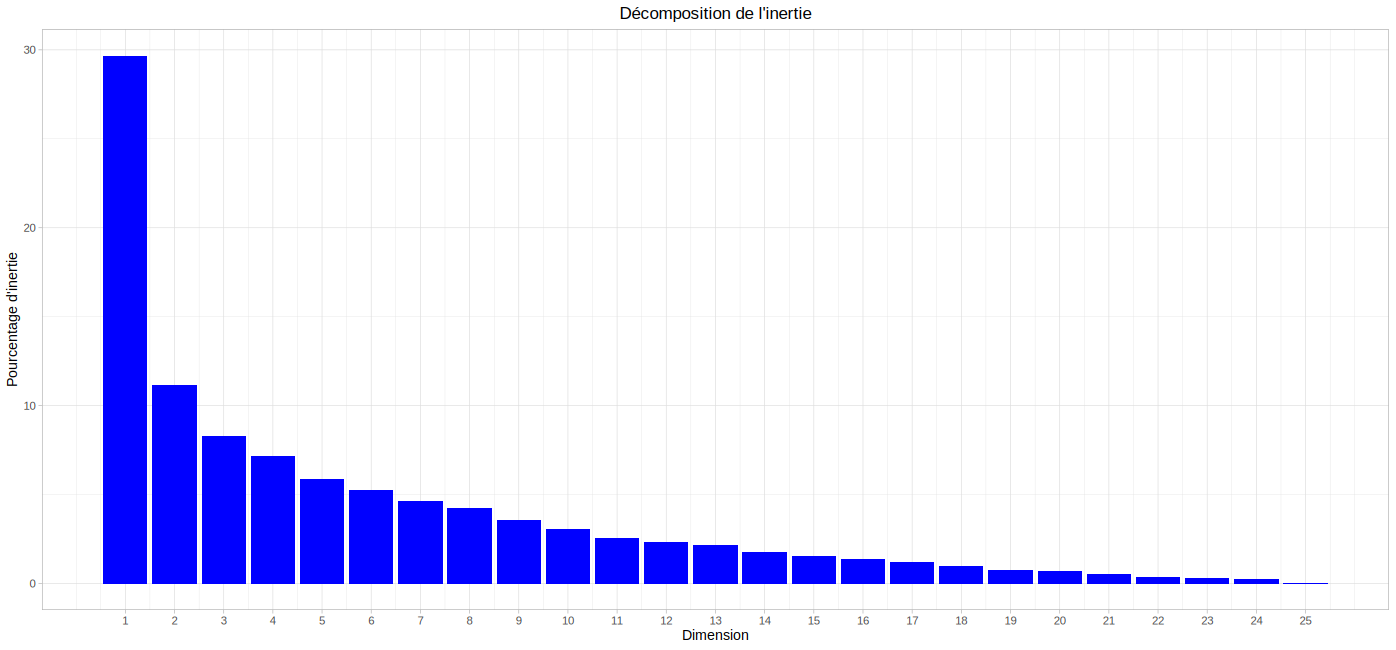
\includegraphics[width=0.5\linewidth]{images/VP2}}

Une ACP de rang pour ce theme permet une analyse plus fine, en réduisant drastiquement l'impact des individus trés attypiques, on peut désormais observer d'autres disparité.\\
En se limitant a \emph  COS2>0,5 \%, on peur désormais mieux éxplorer la structures des villes a faible richesse et attirance observer dans l'ACP normée:

\centerline{\begin{tabular}{ccc}
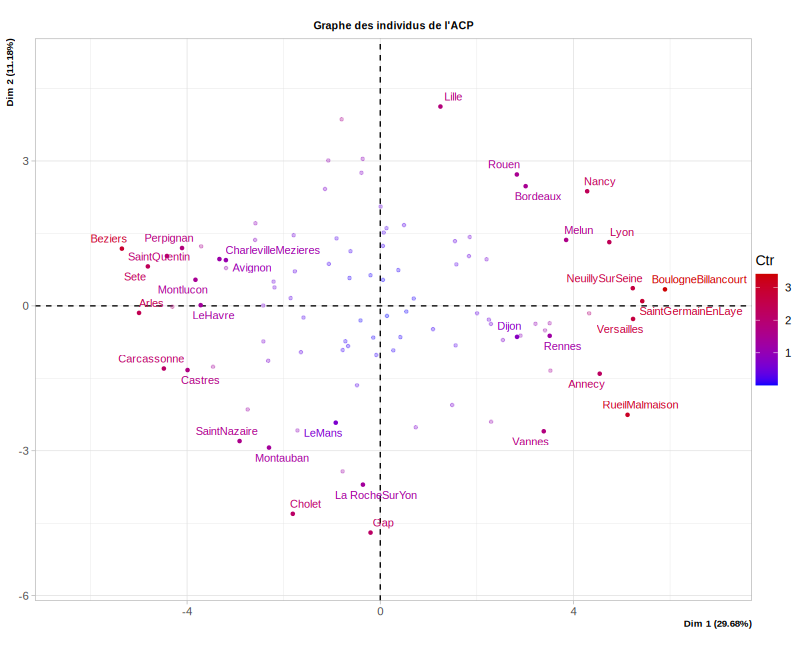
\includegraphics[width=0.6\linewidth]{images/I_2_0,5} &
&
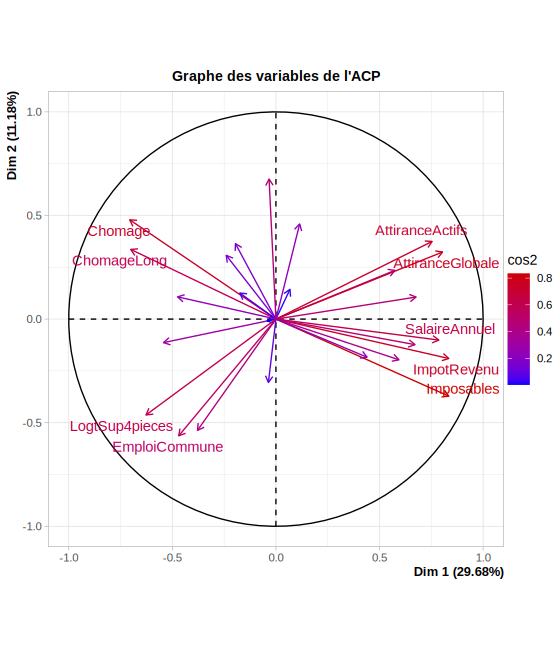
\includegraphics[width=0.3\linewidth]{images/V_2_0,5}
\end{tabular}}


Une premiére partie dans le cadran inferrieur gauche (montauban,cholet,gap...) des villes a haut emplois communal et grand nombre de large habitat (logtsup4piece),et où l'opposition au grandes métropoles se fait moins par leur niveau de richesse que par leur faible capacité a attiré de nouveau habitant.\\
On y retrouve d'ailleur les villes en bordure de zones rurales et d'ancien bassin ouvrier, nous confortant dans cette interprétation.\\

Une deuxieme partie dans le cadran superrieur droit (bezier, perpignon avigon...) des villes a haut taux de chomage et chomage long, et où désormais l'opposition au grandes métropoles se fait moins par leur capacité à attiré de nouveau habitant que par leur faible niveau de richesse.\\

On y retrouve les villes du litoralles, touristique, avec beaucoup d'affluance de retraité, nous confortant dans cette interprétation.\\

Bien que ces différence soit beaucoup moins trancher que pour l'ACP normé, elle suggère de nouvelles dynamiques qui n'étaient pas mis en évidence lorsque la riche region parisenne polariser autant les axes.

\subsection{Thème Risques}

\centerline{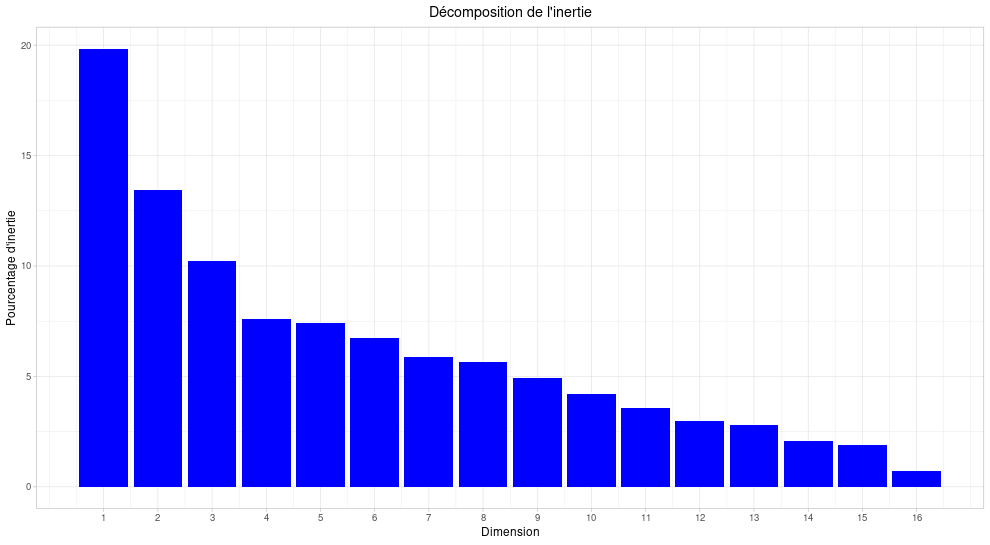
\includegraphics[width=0.8\linewidth]{images/ACPR_ris_vp}}

Il n'y pas de changement notable dans l'étude des valeurs propres. On observe le même décrochement entre la 3-ème et la 4-ème valeur.\\

L'étude des plans (1,2) et (2,3) dont les graphiques se trouvent ci-dessous ne nous montre rien de plus. En effet on retrouve les mêmes faisceaux de variables avec peu ou proue les mêmes villes. Ceci s'explique par le fait qu'il n'y avait pas d'individu singulier par rapport aux variables du thème.

\centerline{\begin{tabular}{ccc}
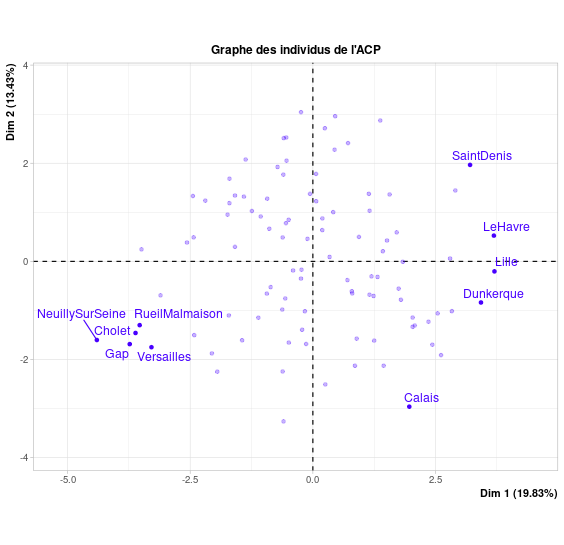
\includegraphics[width=0.55\linewidth]{images/ACPR_ris_ind_12} & 
&
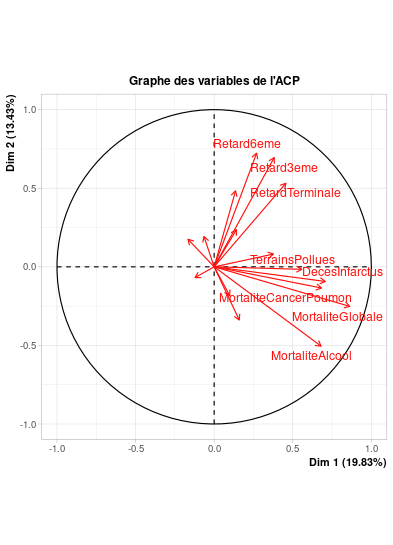
\includegraphics[width=0.40\linewidth]{images/ACPR_ris_var_12}
\end{tabular}}

\centerline{\begin{tabular}{ccc}
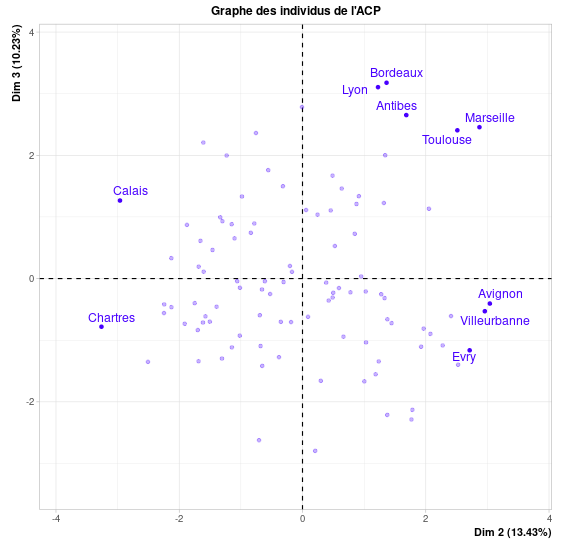
\includegraphics[width=0.55\linewidth]{images/ACPR_ris_ind_23} & 
&
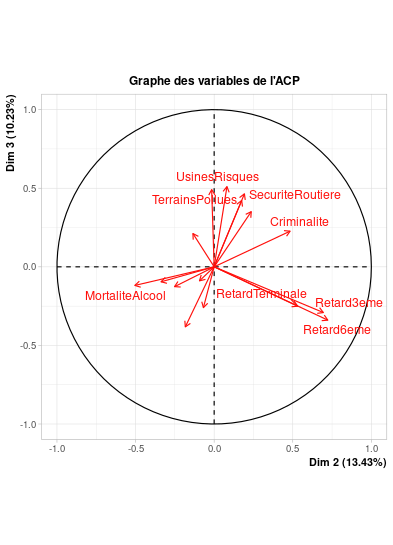
\includegraphics[width=0.40\linewidth]{images/ACPR_ris_var_23}
\end{tabular}}

\subsection{Thème Culture}

Ici, l'acp par rang nous permet, toujours avec 2 axes, de bien mieux observer les disparité entre les villes:


\centerline{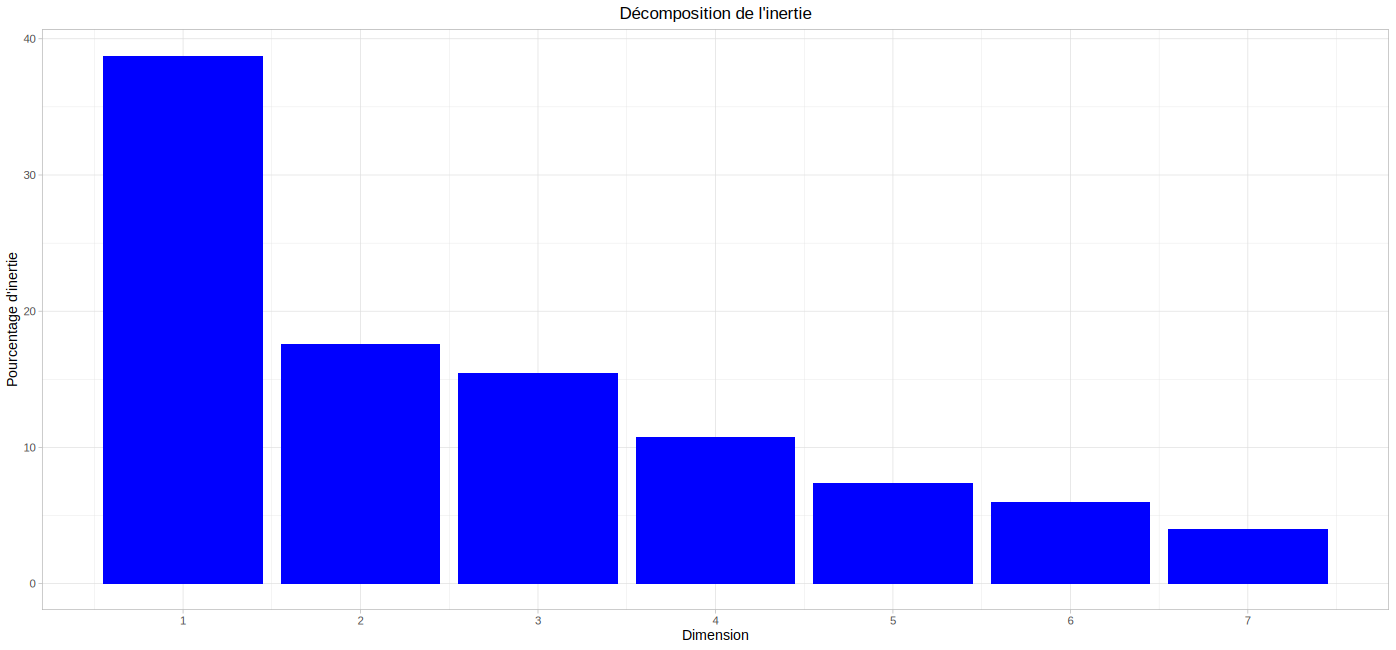
\includegraphics[width=0.8\linewidth]{images/VP4}}

\centerline{\begin{tabular}{ccc}
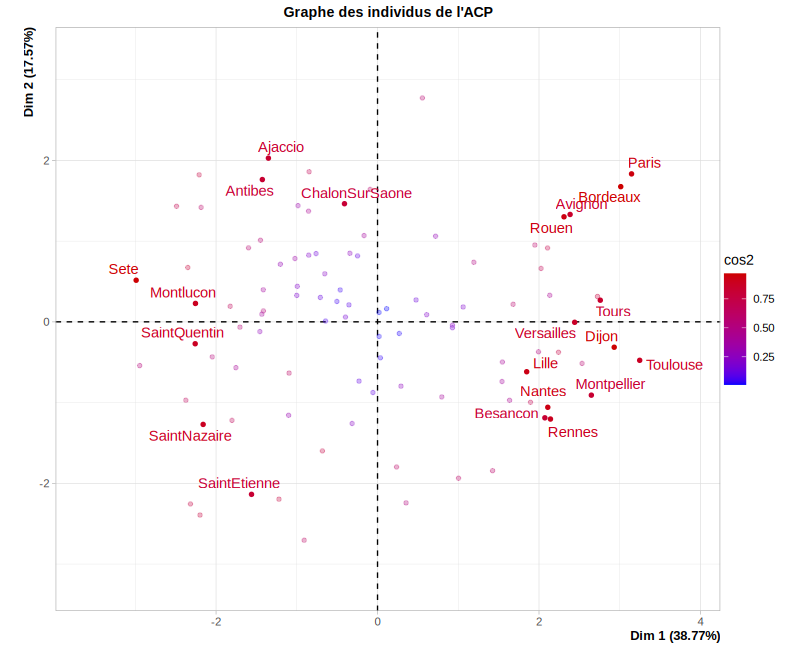
\includegraphics[width=0.6\linewidth]{images/I_4_0,8} &
&
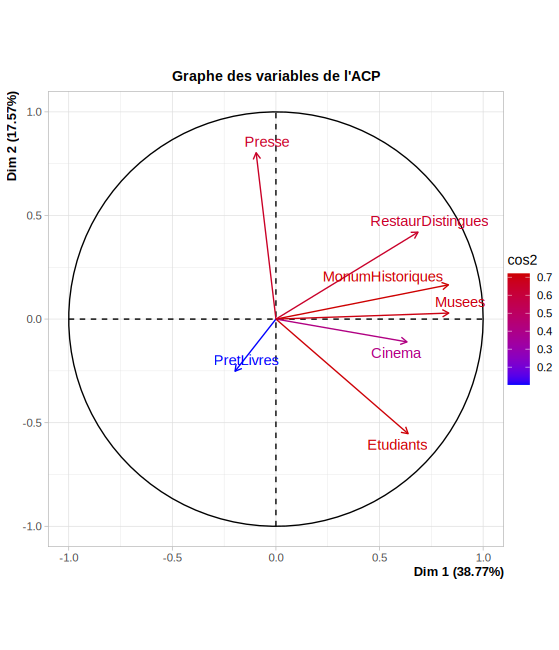
\includegraphics[width=0.3\linewidth]{images/V_4_0,8}
\end{tabular}}

En se limitant a \emph(cos2>0,9)\%, on peut désormé mieux comprendre l'étallement des groupe de villes déterminant la position des variables presse et etudiants :\\
En effet, on découvre alors que les villes (hors paris) ayant de haute valeur pour presse sont majoritairement les villes acceuillant de grands évènement culturel,(canne,angouleme...), villes ne disposant souvent pas des grande infrastructure (grandes écoles, université) pour attiré les millieux etudiants.


\subsection{Thème Nature}

\centerline{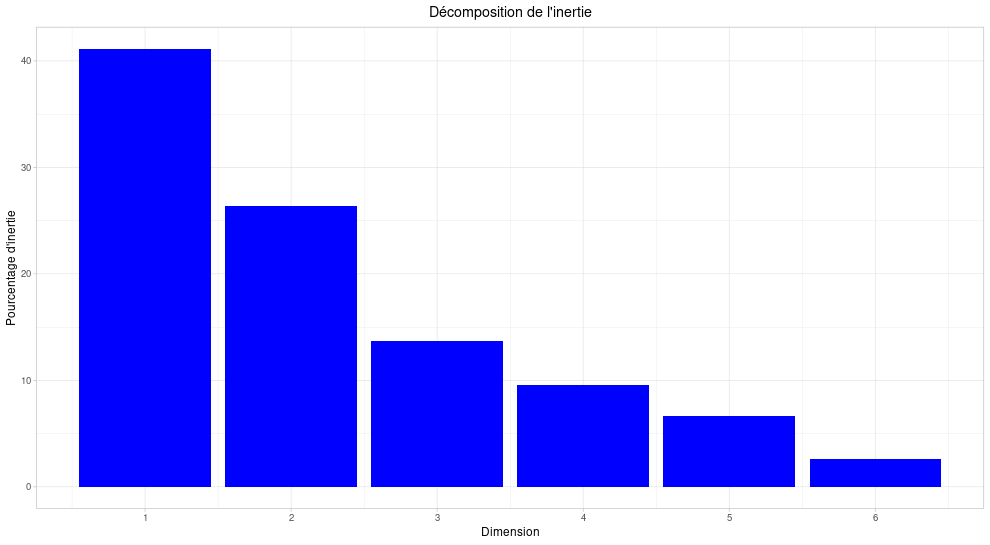
\includegraphics[width=0.8\linewidth]{images/ACPR_nat_vp}}

Bien que l'inertie capturé par les deux premiers axes soit inférieur à celles obtenue lors de l'ACP normée, nous ne garderons de nouveaux que deux axes. Ils capturent 67,49\% de la variance.\\

Certes quelques différences de valeurs apparaissent mais on retrouve sensiblement les mêmes résultats que lors de l'ACP normée, notamment le groupe des villes du Sud et le positionnement opposé sur l'axe deux pour d'un côté des villes typées montagne (Annecy, Gap, Chambéry, Clermont-Ferrand) et de l'autre deux villes de bord de mer (Dunkerque, Quimper, Saint-Nazaire).

\centerline{\begin{tabular}{ccc}
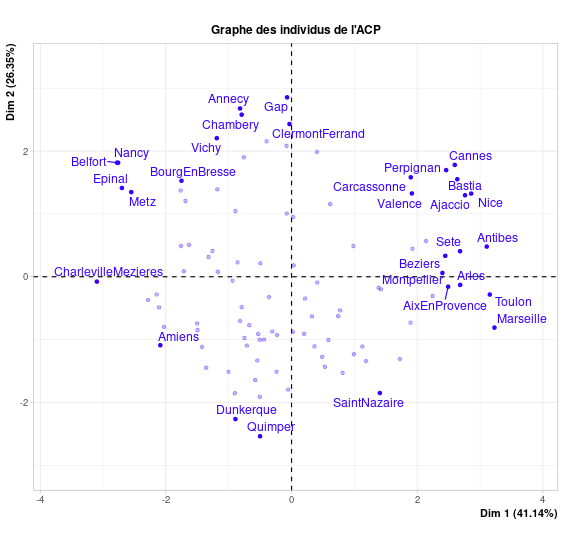
\includegraphics[width=0.55\linewidth]{images/ACPR_nat_ind_12} & 
&
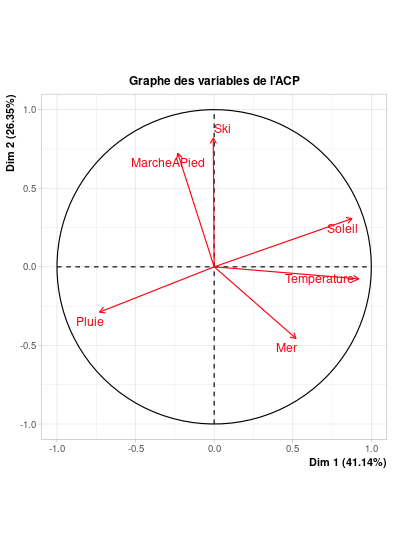
\includegraphics[width=0.40\linewidth]{images/ACPR_nat_var_12}
\end{tabular}}


 
\end{document}
